\subsection{Informacije o isporuci za dostavljača}

Ako dostavljač odabere neku od zakazanih dostava prikazuju mu se detaljnije informacije o toj dostavi (slika \ref{subfig:DeliverymanOrderInfo}).
Ako dostavljač kasni ovde ima mogućnost da obavesti klijenta o tome. Kada se klikne na dugme \textit{Notify about the delay} pojavljuje se forma (slika \ref{subfig:DeliverymanDelay}) gde bi trebalo da unese svoju procenu koliko će kasniti. Sistem automatski šalje mejl korisniku i obaveštava ga o kašnjenju.
Nakon uspešne dostave potrebno je odabrati opciju \textit{Delivered}. Nakog toga sistem čuva da je ova porudžbina dostavljena a dostavljaču se prikazuje poruka koja mu čestita na obavljenoj dostavi i nudi mu mogućnost da se vrati na preostale isporuke (slika \ref{subfig:DeliverymanDone}). Kada se vrati na ekran sa listom svih isporuka, obavljena dostava je obrisana (slika \ref{subfig:DeliverymanListNew}).



\begin{figure}[H]
    \centering
    \subfloat[\centering Ekran detaljnih informacija o isporuci za dostavljača\label{subfig:DeliverymanOrderInfo}]{{	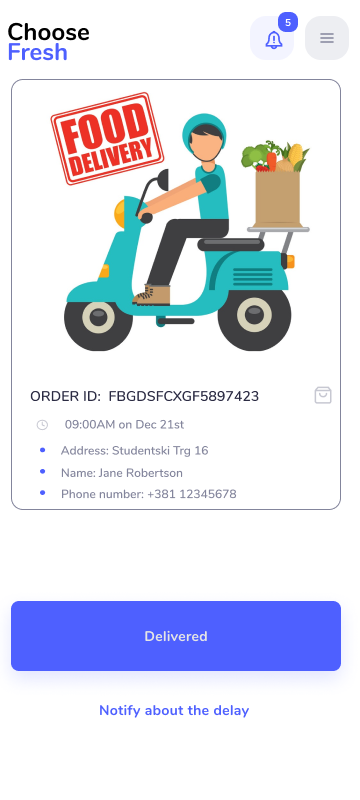
\includegraphics[scale=0.3]{UI/deliveryman_order_info.png}}}
    \qquad
    \subfloat[\centering Ekran za obaveštavanje klijenta o kašnjenju\label{subfig:DeliverymanDelay}]{{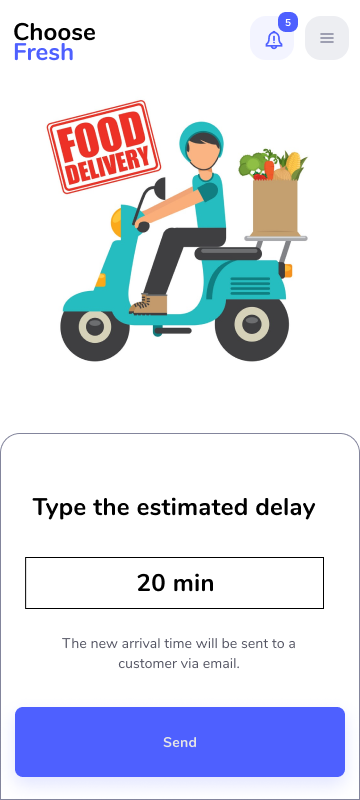
\includegraphics[scale=0.3]{UI/deliveryman_delay_input.png} }}
    
     \centering
    \subfloat[\centering Ekran poruke nakon obavljene dostave\label{subfig:DeliverymanDone}]{{	
\includegraphics[scale=0.3]{UI/deliveryman_done_delivery.png}}}
    \qquad
    \subfloat[\centering Ekran liste zakazanih isporuka dostavljača nakon dostavljanja prve isporuke\label{subfig:DeliverymanListNew}]{{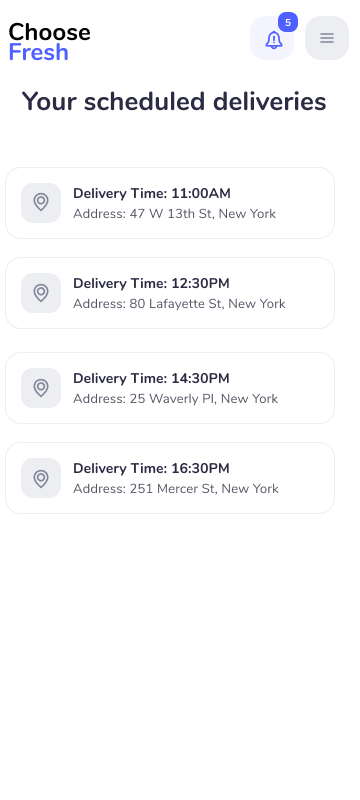
\includegraphics[scale=0.3]{UI/deliveryman_list_of_packages_new.png} }}
    \caption{Ekrani informacije o isporuci za dostavljača}

\end{figure}
